\documentclass[12pt,a4paper]{report}

% ============================================================================
% PACKAGES
% ============================================================================
\usepackage[utf8]{inputenc}
\usepackage[T1]{fontenc}
\usepackage{lmodern}
\usepackage[margin=0.8in]{geometry}
\usepackage{graphicx}
\usepackage{xcolor}
\usepackage{hyperref}
\usepackage{tikz}
\usepackage{longtable}
\usepackage{booktabs}
\usepackage{fancyhdr}
\usepackage{titlesec}
\usepackage{listings}
\usepackage{enumitem}
\usepackage{pdflscape}

% TikZ Libraries
\usetikzlibrary{shapes.geometric, arrows.meta, positioning, fit, backgrounds, 
                er, calc}

% ============================================================================
% COLORS
% ============================================================================
\definecolor{primaryblue}{RGB}{26, 54, 93}
\definecolor{secondaryblue}{RGB}{59, 130, 246}
\definecolor{accentgreen}{RGB}{34, 197, 94}
\definecolor{warningorange}{RGB}{249, 115, 22}
\definecolor{lightgray}{RGB}{243, 244, 246}
\definecolor{darkgray}{RGB}{75, 85, 99}
\definecolor{entitycolor}{RGB}{219, 234, 254}
\definecolor{tablefill}{RGB}{254, 249, 195}

% ============================================================================
% HYPERREF SETUP
% ============================================================================
\hypersetup{
    colorlinks=true,
    linkcolor=primaryblue,
    urlcolor=secondaryblue,
    pdftitle={EduX - Database Schema Documentation},
    pdfauthor={EduX Development Team},
}

% ============================================================================
% HEADER/FOOTER
% ============================================================================
\pagestyle{fancy}
\fancyhf{}
\fancyhead[L]{\textcolor{darkgray}{\small EduX School Management System}}
\fancyhead[R]{\textcolor{darkgray}{\small Database Documentation}}
\fancyfoot[C]{\textcolor{darkgray}{\thepage}}
\renewcommand{\headrulewidth}{0.4pt}

% ============================================================================
% TITLE FORMATTING
% ============================================================================
\titleformat{\chapter}[display]
  {\normalfont\huge\bfseries\color{primaryblue}}
  {\chaptertitlename\ \thechapter}{20pt}{\Huge}

\titleformat{\section}
  {\normalfont\Large\bfseries\color{primaryblue}}
  {\thesection}{1em}{}

\titleformat{\subsection}
  {\normalfont\large\bfseries\color{secondaryblue}}
  {\thesubsection}{1em}{}

% ============================================================================
% LISTINGS SETUP
% ============================================================================
\lstset{
    backgroundcolor=\color{lightgray},
    basicstyle=\ttfamily\footnotesize,
    breaklines=true,
    frame=single,
    rulecolor=\color{darkgray!30},
    language=SQL,
}

% ============================================================================
% DOCUMENT
% ============================================================================
\begin{document}

% ----------------------------------------------------------------------------
% TITLE PAGE
% ----------------------------------------------------------------------------
\begin{titlepage}
    \centering
    \vspace*{2cm}
    
    {\Huge\bfseries\textcolor{primaryblue}{EduX}\par}
    \vspace{0.5cm}
    {\Large\textcolor{secondaryblue}{School Management System}\par}
    
    \vspace{2cm}
    
    
\begin{tikzpicture}
        \node[draw=primaryblue, line width=2pt, rounded corners=10pt, 
              minimum width=8cm, minimum height=3cm, fill=lightgray] 
              {\Huge\bfseries\textcolor{primaryblue}{Database Schema}};
    \end{tikzpicture}
    
    \vspace{1cm}
    {\large\textcolor{darkgray}{\textit{Developer Documentation}}\par}
    
    \vfill
    
    {\large\textcolor{darkgray}{Version 1.0}\par}
    {\large\textcolor{darkgray}{\today}\par}
\end{titlepage}

\tableofcontents
\newpage

% ============================================================================
% CHAPTER 1: OVERVIEW
% ============================================================================
\chapter{Database Overview}

\section{Introduction}

EduX uses SQLite as its database engine, accessed through the Drift ORM (formerly Moor). The database is stored locally on the user's machine, enabling offline-first functionality.

\section{Database Statistics}

\begin{longtable}{@{}p{5cm}p{8cm}@{}}
\toprule
\textbf{Metric} & \textbf{Value} \\
\midrule
\endhead
Total Tables & 27+ \\
Database Engine & SQLite 3 \\
ORM & Drift (dart package) \\
Location & \texttt{AppData/Roaming/EduX/edux\_database.sqlite} \\
\bottomrule
\end{longtable}

\section{Table Categories}

\begin{center}
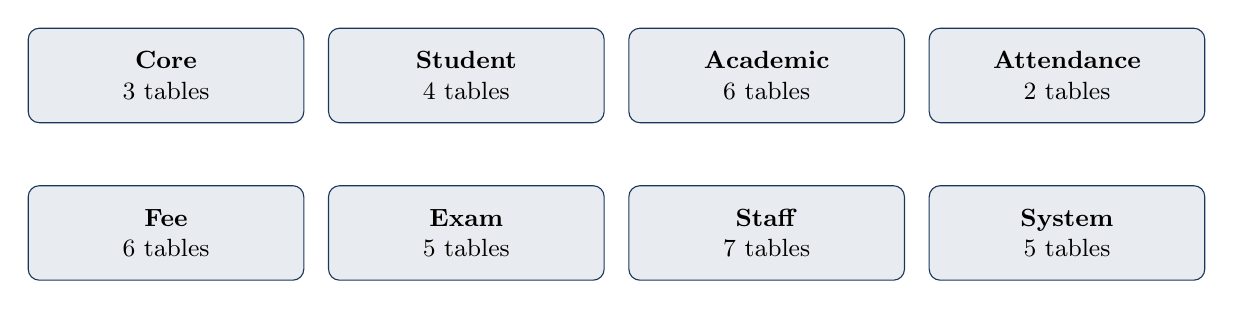
\begin{tikzpicture}[
    cat/.style={draw=primaryblue, rounded corners, minimum width=3.5cm, 
                minimum height=1.2cm, fill=primaryblue!10, align=center, font=\small}
]
    \node[cat] (core) at (0,2) {\textbf{Core}\\3 tables};
    \node[cat, right=0.3cm of core] (student) {\textbf{Student}\\4 tables};
    \node[cat, right=0.3cm of student] (academic) {\textbf{Academic}\\6 tables};
    \node[cat, right=0.3cm of academic] (attendance) {\textbf{Attendance}\\2 tables};
    
    \node[cat] (fee) at (0,0) {\textbf{Fee}\\6 tables};
    \node[cat, right=0.3cm of fee] (exam) {\textbf{Exam}\\5 tables};
    \node[cat, right=0.3cm of exam] (staff) {\textbf{Staff}\\7 tables};
    \node[cat, right=0.3cm of staff] (system) {\textbf{System}\\5 tables};
\end{tikzpicture}
\end{center}

% ============================================================================
% CHAPTER 2: ER DIAGRAM
% ============================================================================
\chapter{Entity Relationship Diagram}

\section{Complete ER Diagram}

\begin{landscape}
\begin{center}
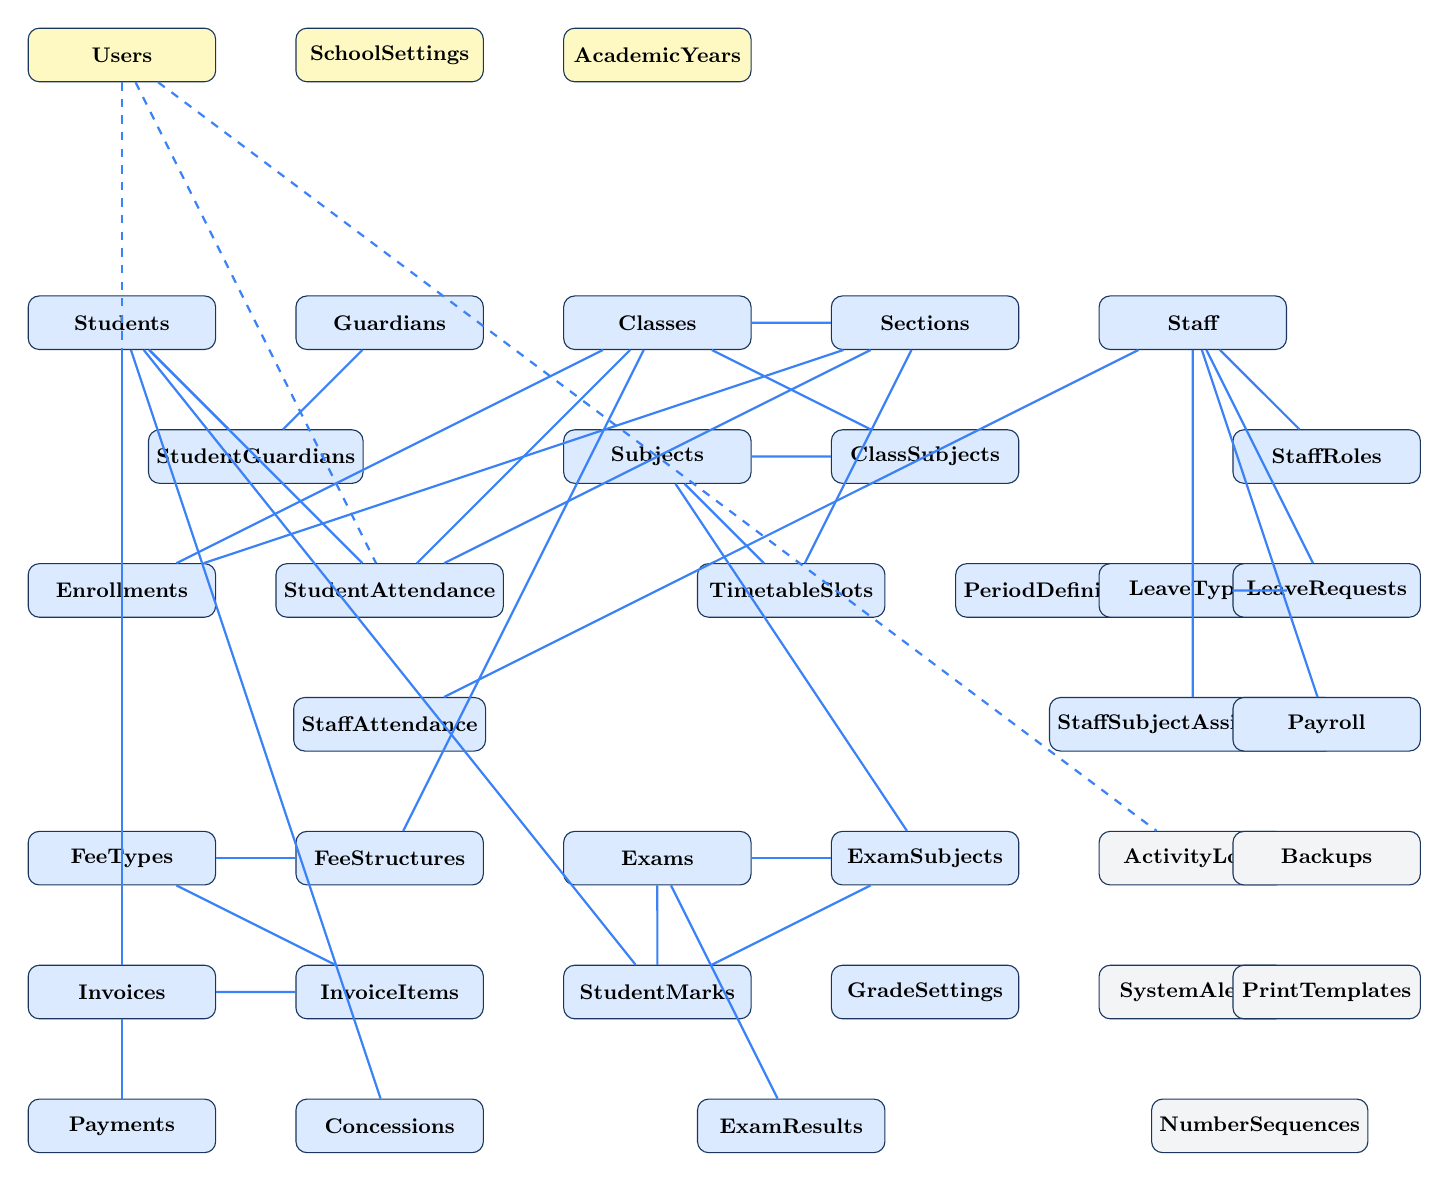
\begin{tikzpicture}[
    entity/.style={draw=primaryblue, rounded corners, minimum width=2.8cm, 
                   minimum height=0.8cm, fill=entitycolor, font=\small\bfseries},
    relation/.style={draw=secondaryblue, thick},
    scale=0.85, transform shape
]
    % ==================== CORE TABLES ====================
    \node[entity, fill=tablefill] (users) at (0,12) {Users};
    \node[entity, fill=tablefill] (school) at (4,12) {SchoolSettings};
    \node[entity, fill=tablefill] (years) at (8,12) {AcademicYears};
    
    % ==================== STUDENT TABLES ====================
    \node[entity] (students) at (0,8) {Students};
    \node[entity] (guardians) at (4,8) {Guardians};
    \node[entity] (studguard) at (2,6) {StudentGuardians};
    \node[entity] (enrollments) at (0,4) {Enrollments};
    
    % ==================== ACADEMIC TABLES ====================
    \node[entity] (classes) at (8,8) {Classes};
    \node[entity] (sections) at (12,8) {Sections};
    \node[entity] (subjects) at (8,6) {Subjects};
    \node[entity] (classubj) at (12,6) {ClassSubjects};
    \node[entity] (timetable) at (10,4) {TimetableSlots};
    \node[entity] (periods) at (14,4) {PeriodDefinitions};
    
    % ==================== ATTENDANCE TABLES ====================
    \node[entity] (studatt) at (4,4) {StudentAttendance};
    \node[entity] (staffatt) at (4,2) {StaffAttendance};
    
    % ==================== FEE TABLES ====================
    \node[entity] (feetypes) at (0,0) {FeeTypes};
    \node[entity] (feestructs) at (4,0) {FeeStructures};
    \node[entity] (invoices) at (0,-2) {Invoices};
    \node[entity] (invitems) at (4,-2) {InvoiceItems};
    \node[entity] (payments) at (0,-4) {Payments};
    \node[entity] (concessions) at (4,-4) {Concessions};
    
    % ==================== EXAM TABLES ====================
    \node[entity] (exams) at (8,0) {Exams};
    \node[entity] (examsubj) at (12,0) {ExamSubjects};
    \node[entity] (marks) at (8,-2) {StudentMarks};
    \node[entity] (grades) at (12,-2) {GradeSettings};
    \node[entity] (results) at (10,-4) {ExamResults};
    
    % ==================== STAFF TABLES ====================
    \node[entity] (staff) at (16,8) {Staff};
    \node[entity] (roles) at (18,6) {StaffRoles};
    \node[entity] (leavetypes) at (16,4) {LeaveTypes};
    \node[entity] (leavereq) at (18,4) {LeaveRequests};
    \node[entity] (assign) at (16,2) {StaffSubjectAssignments};
    \node[entity] (payroll) at (18,2) {Payroll};
    
    % ==================== SYSTEM TABLES ====================
    \node[entity, fill=lightgray] (logs) at (16,0) {ActivityLogs};
    \node[entity, fill=lightgray] (backups) at (18,0) {Backups};
    \node[entity, fill=lightgray] (alerts) at (16,-2) {SystemAlerts};
    \node[entity, fill=lightgray] (templates) at (18,-2) {PrintTemplates};
    \node[entity, fill=lightgray] (sequences) at (17,-4) {NumberSequences};
    
    % ==================== RELATIONSHIPS ====================
    % Student relationships
    \draw[relation] (students) -- (studguard);
    \draw[relation] (guardians) -- (studguard);
    \draw[relation] (students) -- (enrollments);
    \draw[relation] (students) -- (studatt);
    \draw[relation] (students) -- (invoices);
    \draw[relation] (students) -- (marks);
    \draw[relation] (students) -- (concessions);
    
    % Academic relationships
    \draw[relation] (classes) -- (sections);
    \draw[relation] (classes) -- (classubj);
    \draw[relation] (subjects) -- (classubj);
    \draw[relation] (sections) -- (timetable);
    \draw[relation] (subjects) -- (timetable);
    \draw[relation] (enrollments) -- (classes);
    \draw[relation] (enrollments) -- (sections);
    
    % Attendance relationships
    \draw[relation] (studatt) -- (classes);
    \draw[relation] (studatt) -- (sections);
    \draw[relation] (staffatt) -- (staff);
    
    % Fee relationships
    \draw[relation] (feetypes) -- (feestructs);
    \draw[relation] (classes) -- (feestructs);
    \draw[relation] (invoices) -- (invitems);
    \draw[relation] (feetypes) -- (invitems);
    \draw[relation] (invoices) -- (payments);
    
    % Exam relationships
    \draw[relation] (exams) -- (examsubj);
    \draw[relation] (subjects) -- (examsubj);
    \draw[relation] (exams) -- (marks);
    \draw[relation] (examsubj) -- (marks);
    \draw[relation] (exams) -- (results);
    
    % Staff relationships
    \draw[relation] (staff) -- (roles);
    \draw[relation] (staff) -- (leavereq);
    \draw[relation] (leavetypes) -- (leavereq);
    \draw[relation] (staff) -- (assign);
    \draw[relation] (staff) -- (payroll);
    
    % User relationships
    \draw[relation, dashed] (users) -- (studatt);
    \draw[relation, dashed] (users) -- (invoices);
    \draw[relation, dashed] (users) -- (logs);
\end{tikzpicture}
\end{center}
\end{landscape}

% ============================================================================
% CHAPTER 3: CORE TABLES
% ============================================================================
\chapter{Core Tables}

\section{SchoolSettings}

Stores school configuration and settings.

\begin{longtable}{@{}p{4cm}p{2.5cm}p{6.5cm}@{}}
\toprule
\textbf{Column} & \textbf{Type} & \textbf{Description} \\
\midrule
\endhead
id & INTEGER & Primary key (auto-increment) \\
schoolName & TEXT & School name (max 200 chars) \\
logo & BLOB & School logo image \\
address & TEXT & School address \\
city & TEXT & City \\
state & TEXT & State/Province \\
postalCode & TEXT & Postal code \\
country & TEXT & Country (default: Pakistan) \\
phone & TEXT & Primary phone \\
email & TEXT & Email address \\
principalName & TEXT & Principal's name \\
currencySymbol & TEXT & Currency (default: PKR) \\
currentAcademicYear & TEXT & Current year (e.g., 2025-2026) \\
workingDays & TEXT & Comma-separated days \\
schoolStartTime & TEXT & HH:mm format \\
schoolEndTime & TEXT & HH:mm format \\
isSetupComplete & BOOLEAN & Setup wizard completed \\
createdAt & DATETIME & Record creation time \\
updatedAt & DATETIME & Last update time \\
\bottomrule
\end{longtable}

\section{Users}

User accounts with authentication.

\begin{longtable}{@{}p{4cm}p{2.5cm}p{6.5cm}@{}}
\toprule
\textbf{Column} & \textbf{Type} & \textbf{Description} \\
\midrule
\endhead
id & INTEGER & Primary key \\
uuid & TEXT & Unique external identifier \\
username & TEXT & Login username (unique) \\
passwordHash & TEXT & SHA-256 password hash \\
passwordSalt & TEXT & Password salt \\
fullName & TEXT & Display name \\
email & TEXT & Email address \\
phone & TEXT & Phone number \\
role & TEXT & admin/principal/teacher/accountant \\
photo & BLOB & Profile photo \\
isActive & BOOLEAN & Account active status \\
isSystemAdmin & BOOLEAN & Cannot be deleted \\
lastLogin & DATETIME & Last login timestamp \\
createdAt & DATETIME & Creation time \\
updatedAt & DATETIME & Update time \\
\bottomrule
\end{longtable}

\section{AcademicYears}

Academic year configurations.

\begin{longtable}{@{}p{4cm}p{2.5cm}p{6.5cm}@{}}
\toprule
\textbf{Column} & \textbf{Type} & \textbf{Description} \\
\midrule
\endhead
id & INTEGER & Primary key \\
name & TEXT & Year name (e.g., 2025-2026) \\
startDate & DATETIME & Year start date \\
endDate & DATETIME & Year end date \\
isCurrent & BOOLEAN & Currently active year \\
isArchived & BOOLEAN & Archived status \\
createdAt & DATETIME & Creation time \\
\bottomrule
\end{longtable}

% ============================================================================
% CHAPTER 4: STUDENT TABLES
% ============================================================================
\chapter{Student Tables}

\section{Students}

Complete student information.

\begin{longtable}{@{}p{4cm}p{2.5cm}p{6.5cm}@{}}
\toprule
\textbf{Column} & \textbf{Type} & \textbf{Description} \\
\midrule
\endhead
id & INTEGER & Primary key \\
uuid & TEXT & Unique identifier \\
admissionNumber & TEXT & Unique admission number \\
firstName & TEXT & First name (1-50 chars) \\
lastName & TEXT & Last name (1-50 chars) \\
dateOfBirth & DATETIME & Birth date \\
gender & TEXT & male/female \\
bloodGroup & TEXT & Blood group \\
religion & TEXT & Religion \\
nationality & TEXT & Nationality (default: Pakistani) \\
cnic & TEXT & CNIC/B-Form number \\
address & TEXT & Residential address \\
city & TEXT & City \\
phone & TEXT & Contact phone \\
email & TEXT & Email address \\
photo & BLOB & Student photo \\
medicalInfo & TEXT & Medical notes \\
allergies & TEXT & Known allergies \\
specialNeeds & TEXT & Special requirements \\
previousSchool & TEXT & Previous school name \\
status & TEXT & active/inactive/graduated/withdrawn \\
admissionDate & DATETIME & Admission date \\
leavingDate & DATETIME & Leaving date (if applicable) \\
leavingReason & TEXT & Reason for leaving \\
notes & TEXT & Additional notes \\
createdAt & DATETIME & Creation time \\
updatedAt & DATETIME & Update time \\
\bottomrule
\end{longtable}

\section{Guardians}

Parent/Guardian information.

\begin{longtable}{@{}p{4cm}p{2.5cm}p{6.5cm}@{}}
\toprule
\textbf{Column} & \textbf{Type} & \textbf{Description} \\
\midrule
\endhead
id & INTEGER & Primary key \\
uuid & TEXT & Unique identifier \\
firstName & TEXT & First name \\
lastName & TEXT & Last name \\
relation & TEXT & father/mother/guardian/other \\
cnic & TEXT & CNIC number \\
phone & TEXT & Primary phone (required) \\
alternatePhone & TEXT & Secondary phone \\
email & TEXT & Email address \\
occupation & TEXT & Job/Profession \\
workplace & TEXT & Employer name \\
address & TEXT & Address \\
city & TEXT & City \\
photo & BLOB & Guardian photo \\
createdAt & DATETIME & Creation time \\
updatedAt & DATETIME & Update time \\
\bottomrule
\end{longtable}

\section{StudentGuardians}

Many-to-many relationship between students and guardians.

\begin{longtable}{@{}p{4cm}p{2.5cm}p{6.5cm}@{}}
\toprule
\textbf{Column} & \textbf{Type} & \textbf{Description} \\
\midrule
\endhead
studentId & INTEGER & FK to Students (cascade delete) \\
guardianId & INTEGER & FK to Guardians (cascade delete) \\
isPrimary & BOOLEAN & Primary guardian flag \\
canPickup & BOOLEAN & Can pickup student \\
isEmergencyContact & BOOLEAN & Emergency contact flag \\
createdAt & DATETIME & Creation time \\
\multicolumn{3}{l}{\textit{Primary Key: (studentId, guardianId)}} \\
\bottomrule
\end{longtable}

\section{Enrollments}

Student class enrollment history.

\begin{longtable}{@{}p{4cm}p{2.5cm}p{6.5cm}@{}}
\toprule
\textbf{Column} & \textbf{Type} & \textbf{Description} \\
\midrule
\endhead
id & INTEGER & Primary key \\
studentId & INTEGER & FK to Students \\
classId & INTEGER & FK to Classes \\
sectionId & INTEGER & FK to Sections \\
academicYear & TEXT & Academic year \\
rollNumber & TEXT & Roll number in class \\
enrollmentDate & DATETIME & Enrollment date \\
endDate & DATETIME & End date (if applicable) \\
status & TEXT & active/promoted/transferred/withdrawn \\
isCurrent & BOOLEAN & Current enrollment flag \\
notes & TEXT & Notes about enrollment \\
createdAt & DATETIME & Creation time \\
updatedAt & DATETIME & Update time \\
\bottomrule
\end{longtable}

% ============================================================================
% CHAPTER 5: ACADEMIC TABLES
% ============================================================================
\chapter{Academic Tables}

\section{Classes}

School class definitions.

\begin{longtable}{@{}p{4cm}p{2.5cm}p{6.5cm}@{}}
\toprule
\textbf{Column} & \textbf{Type} & \textbf{Description} \\
\midrule
\endhead
id & INTEGER & Primary key \\
name & TEXT & Class name (e.g., Class 5) \\
level & TEXT & pre\_primary/primary/middle/secondary \\
gradeLevel & INTEGER & Numeric level for sorting \\
displayOrder & INTEGER & Display order \\
description & TEXT & Class description \\
monthlyFee & REAL & Default monthly fee \\
isActive & BOOLEAN & Active status \\
createdAt & DATETIME & Creation time \\
updatedAt & DATETIME & Update time \\
\bottomrule
\end{longtable}

\section{Sections}

Class sections (A, B, C, etc.).

\begin{longtable}{@{}p{4cm}p{2.5cm}p{6.5cm}@{}}
\toprule
\textbf{Column} & \textbf{Type} & \textbf{Description} \\
\midrule
\endhead
id & INTEGER & Primary key \\
classId & INTEGER & FK to Classes \\
name & TEXT & Section name (e.g., A) \\
capacity & INTEGER & Maximum students \\
classTeacherId & INTEGER & FK to Staff (optional) \\
roomNumber & TEXT & Room number/name \\
isActive & BOOLEAN & Active status \\
createdAt & DATETIME & Creation time \\
updatedAt & DATETIME & Update time \\
\bottomrule
\end{longtable}

\section{Subjects}

Subject definitions.

\begin{longtable}{@{}p{4cm}p{2.5cm}p{6.5cm}@{}}
\toprule
\textbf{Column} & \textbf{Type} & \textbf{Description} \\
\midrule
\endhead
id & INTEGER & Primary key \\
code & TEXT & Subject code (e.g., ENG) \\
name & TEXT & Subject name \\
type & TEXT & core/elective/optional \\
creditHours & INTEGER & Credit hours per week \\
description & TEXT & Description \\
isActive & BOOLEAN & Active status \\
createdAt & DATETIME & Creation time \\
updatedAt & DATETIME & Update time \\
\bottomrule
\end{longtable}

% ============================================================================
% CHAPTER 6: FEE TABLES
% ============================================================================
\chapter{Fee Tables}

\section{FeeTypes}

Fee category definitions.

\begin{longtable}{@{}p{4cm}p{2.5cm}p{6.5cm}@{}}
\toprule
\textbf{Column} & \textbf{Type} & \textbf{Description} \\
\midrule
\endhead
id & INTEGER & Primary key \\
name & TEXT & Fee type name \\
description & TEXT & Description \\
isMonthly & BOOLEAN & Monthly recurring fee \\
isRefundable & BOOLEAN & Refundable fee \\
accountCode & TEXT & Accounting code \\
isActive & BOOLEAN & Active status \\
displayOrder & INTEGER & Display order \\
createdAt & DATETIME & Creation time \\
updatedAt & DATETIME & Update time \\
\bottomrule
\end{longtable}

\section{Invoices}

Fee invoices.

\begin{longtable}{@{}p{4cm}p{2.5cm}p{6.5cm}@{}}
\toprule
\textbf{Column} & \textbf{Type} & \textbf{Description} \\
\midrule
\endhead
id & INTEGER & Primary key \\
invoiceNumber & TEXT & Unique invoice number \\
studentId & INTEGER & FK to Students \\
month & TEXT & Invoice month (YYYY-MM) \\
academicYear & TEXT & Academic year \\
totalAmount & REAL & Sum of all fee items \\
discountAmount & REAL & Discount from concessions \\
netAmount & REAL & Total - discount \\
paidAmount & REAL & Amount paid so far \\
balanceAmount & REAL & Net - paid \\
status & TEXT & pending/partial/paid/overdue \\
issueDate & DATETIME & Invoice issue date \\
dueDate & DATETIME & Payment due date \\
lastPaymentDate & DATETIME & Last payment date \\
notes & TEXT & Notes \\
generatedBy & INTEGER & FK to Users \\
createdAt & DATETIME & Creation time \\
updatedAt & DATETIME & Update time \\
\bottomrule
\end{longtable}

\section{Payments}

Payment transactions.

\begin{longtable}{@{}p{4cm}p{2.5cm}p{6.5cm}@{}}
\toprule
\textbf{Column} & \textbf{Type} & \textbf{Description} \\
\midrule
\endhead
id & INTEGER & Primary key \\
receiptNumber & TEXT & Unique receipt number \\
invoiceId & INTEGER & FK to Invoices \\
studentId & INTEGER & FK to Students \\
amount & REAL & Payment amount \\
paymentMode & TEXT & cash/bank\_transfer/cheque/online \\
referenceNumber & TEXT & Transaction reference \\
bankName & TEXT & Bank name \\
chequeDate & DATETIME & Cheque date \\
remarks & TEXT & Payment remarks \\
paymentDate & DATETIME & Payment date \\
receivedBy & INTEGER & FK to Users \\
isCancelled & BOOLEAN & Cancelled flag \\
cancellationReason & TEXT & Cancellation reason \\
createdAt & DATETIME & Creation time \\
updatedAt & DATETIME & Update time \\
\bottomrule
\end{longtable}

% ============================================================================
% CHAPTER 7: EXAM TABLES
% ============================================================================
\chapter{Examination Tables}

\section{Exams}

Exam definitions.

\begin{longtable}{@{}p{4cm}p{2.5cm}p{6.5cm}@{}}
\toprule
\textbf{Column} & \textbf{Type} & \textbf{Description} \\
\midrule
\endhead
id & INTEGER & Primary key \\
uuid & TEXT & Unique identifier \\
name & TEXT & Exam name \\
type & TEXT & unit\_test/term\_exam/annual\_exam \\
academicYear & TEXT & Academic year \\
classId & INTEGER & FK to Classes \\
startDate & DATETIME & Exam start date \\
endDate & DATETIME & Exam end date \\
description & TEXT & Description \\
status & TEXT & draft/active/completed \\
createdBy & INTEGER & FK to Users \\
createdAt & DATETIME & Creation time \\
updatedAt & DATETIME & Update time \\
\bottomrule
\end{longtable}

\section{StudentMarks}

Marks obtained by students.

\begin{longtable}{@{}p{4cm}p{2.5cm}p{6.5cm}@{}}
\toprule
\textbf{Column} & \textbf{Type} & \textbf{Description} \\
\midrule
\endhead
id & INTEGER & Primary key \\
examId & INTEGER & FK to Exams \\
examSubjectId & INTEGER & FK to ExamSubjects \\
studentId & INTEGER & FK to Students \\
marksObtained & REAL & Marks obtained \\
isAbsent & BOOLEAN & Absent flag \\
grade & TEXT & Calculated grade \\
remarks & TEXT & Remarks \\
enteredBy & INTEGER & FK to Users \\
createdAt & DATETIME & Creation time \\
updatedAt & DATETIME & Update time \\
\multicolumn{3}{l}{\textit{Unique: (examSubjectId, studentId)}} \\
\bottomrule
\end{longtable}

\section{GradeSettings}

Grading criteria.

\begin{longtable}{@{}p{4cm}p{2.5cm}p{6.5cm}@{}}
\toprule
\textbf{Column} & \textbf{Type} & \textbf{Description} \\
\midrule
\endhead
id & INTEGER & Primary key \\
grade & TEXT & Grade name (e.g., A+) \\
minPercentage & REAL & Minimum percentage \\
maxPercentage & REAL & Maximum percentage \\
gpa & REAL & GPA points \\
remarks & TEXT & Report card remarks \\
displayOrder & INTEGER & Display order \\
isPassing & BOOLEAN & Passing grade flag \\
createdAt & DATETIME & Creation time \\
updatedAt & DATETIME & Update time \\
\bottomrule
\end{longtable}

% ============================================================================
% CHAPTER 8: STAFF TABLES
% ============================================================================
\chapter{Staff Tables}

\section{Staff}

Employee information.

\begin{longtable}{@{}p{4cm}p{2.5cm}p{6.5cm}@{}}
\toprule
\textbf{Column} & \textbf{Type} & \textbf{Description} \\
\midrule
\endhead
id & INTEGER & Primary key \\
uuid & TEXT & Unique identifier \\
employeeId & TEXT & Unique employee ID \\
firstName & TEXT & First name \\
lastName & TEXT & Last name \\
dateOfBirth & DATETIME & Birth date \\
gender & TEXT & male/female \\
cnic & TEXT & CNIC number \\
phone & TEXT & Primary phone \\
email & TEXT & Email address \\
address & TEXT & Address \\
qualification & TEXT & Highest qualification \\
specialization & TEXT & Subject expertise \\
designation & TEXT & Job title \\
department & TEXT & Department \\
roleId & INTEGER & FK to StaffRoles \\
basicSalary & REAL & Monthly basic salary \\
joiningDate & DATETIME & Joining date \\
status & TEXT & active/on\_leave/resigned \\
userId & INTEGER & FK to Users (optional) \\
createdAt & DATETIME & Creation time \\
updatedAt & DATETIME & Update time \\
\bottomrule
\end{longtable}

\section{Payroll}

Salary records.

\begin{longtable}{@{}p{4cm}p{2.5cm}p{6.5cm}@{}}
\toprule
\textbf{Column} & \textbf{Type} & \textbf{Description} \\
\midrule
\endhead
id & INTEGER & Primary key \\
staffId & INTEGER & FK to Staff \\
month & TEXT & Payroll month (YYYY-MM) \\
basicSalary & REAL & Basic salary \\
allowances & REAL & Total allowances \\
deductions & REAL & Total deductions \\
netSalary & REAL & Net salary \\
workingDays & INTEGER & Working days in month \\
daysPresent & INTEGER & Days present \\
daysAbsent & INTEGER & Days absent \\
leaveDays & INTEGER & Paid leave days \\
status & TEXT & pending/paid \\
paidDate & DATETIME & Payment date \\
paymentMode & TEXT & cash/bank\_transfer/cheque \\
processedBy & INTEGER & FK to Users \\
createdAt & DATETIME & Creation time \\
\multicolumn{3}{l}{\textit{Unique: (staffId, month)}} \\
\bottomrule
\end{longtable}

% ============================================================================
% CHAPTER 9: SYSTEM TABLES
% ============================================================================
\chapter{System Tables}

\section{ActivityLogs}

Audit trail for all actions.

\begin{longtable}{@{}p{4cm}p{2.5cm}p{6.5cm}@{}}
\toprule
\textbf{Column} & \textbf{Type} & \textbf{Description} \\
\midrule
\endhead
id & INTEGER & Primary key \\
userId & INTEGER & FK to Users (nullable) \\
action & TEXT & login/logout/create/update/delete \\
module & TEXT & Module name \\
entityType & TEXT & Entity type (student, etc.) \\
entityId & INTEGER & Affected entity ID \\
description & TEXT & Action description \\
details & TEXT & Additional details (JSON) \\
previousValues & TEXT & Previous values (JSON) \\
newValues & TEXT & New values (JSON) \\
createdAt & DATETIME & Timestamp \\
\bottomrule
\end{longtable}

\section{Backups}

Backup metadata.

\begin{longtable}{@{}p{4cm}p{2.5cm}p{6.5cm}@{}}
\toprule
\textbf{Column} & \textbf{Type} & \textbf{Description} \\
\midrule
\endhead
id & INTEGER & Primary key \\
fileName & TEXT & Backup file name \\
filePath & TEXT & Full file path \\
fileSize & INTEGER & Size in bytes \\
type & TEXT & manual/auto \\
description & TEXT & Backup notes \\
dbVersion & INTEGER & Database version \\
appVersion & TEXT & App version \\
studentCount & INTEGER & Students at backup time \\
staffCount & INTEGER & Staff at backup time \\
createdBy & INTEGER & FK to Users \\
isValid & BOOLEAN & Backup verified \\
createdAt & DATETIME & Backup timestamp \\
\bottomrule
\end{longtable}

\section{NumberSequences}

Sequential number generation.

\begin{longtable}{@{}p{4cm}p{2.5cm}p{6.5cm}@{}}
\toprule
\textbf{Column} & \textbf{Type} & \textbf{Description} \\
\midrule
\endhead
id & INTEGER & Primary key \\
name & TEXT & Sequence name (unique) \\
prefix & TEXT & Number prefix \\
suffix & TEXT & Number suffix \\
currentNumber & INTEGER & Current sequence value \\
minDigits & INTEGER & Minimum digits (pad zeros) \\
resetPeriod & TEXT & never/yearly/monthly \\
lastResetDate & DATETIME & Last reset date \\
includeYear & BOOLEAN & Include year in number \\
includeMonth & BOOLEAN & Include month in number \\
createdAt & DATETIME & Creation time \\
updatedAt & DATETIME & Update time \\
\bottomrule
\end{longtable}

\end{document}
